\section{Theorie}
\label{sec:Theorie}

Zur Bestimmung beliebiger unbekannter physikalisher Größen, die sich eindeutig als elektrischer Widerstand darstellen lassen, eignen sich vor allem Brückenschaltungen, die im Folgenden näher beschrieben werden sollen. 
In Brückenschaltungen nutzt man die von den Widerstandsverhältnissen abhängige Potentialdifferenz zwischen zwei getrennten stromdurchflossenen Leitern. Das grundsätzliche Schema einer solchen Brückenschaltung ist in \autoref{fig:prinzbrückscha} dargestellt.

\begin{figure}[H]
    \centering
    \includegraphics{figures/Prinzipielle Brückenschaltung.pdf}
    \caption{Darstellung einer prinzipiellen Brückenschaltung\cite{ap07}.}
    \label{fig:prinzbrückscha}
\end{figure}

Die Potentialdifferenz zwischen den Punkten A und B wird als \textbf{Brückenspannung} bezeichnet, zu deren Berechnung die Kirchhoffschen Gesetze genutzt werden.

Mit 
\begin{equation}
    \sum_kI_k = 0
    \label{eq:kirchhoff1}
\end{equation}
und 
\begin{equation}
    \sum_k E_k = \sum_k I_k R_k \,,
    \label{eq:kirchhoff2}
\end{equation} wobei $E_k$ die elektromotorische Kraft darstellt,
ergeben sich folgende Beziehungen:

\begin{equation*}
    I_1 = I_2
\end{equation*}
und
\begin{equation*}
    I_3 = I_4
\end{equation*}

sowie

\begin{equation}
    U = -R_1 I_1 + R_3 I_3
    \label{eq:spannungglei1}
\end{equation}
und
\begin{equation}
    -U = -R_2 I_2 + R_4 I_4 \,.
    \label{eq:spannungglei2}
\end{equation}

Durch Ausnutzen von $I_2 = I_1$ und $I_3 = I_4$ ergibt sich in \eqref{eq:spannungglei2}
\begin{equation}
    -U = -R_2 I_1 + R_4 I_3
    \label{eq:spannungglei3} \,, 
\end{equation}
mit \eqref{eq:spannungglei1} und \eqref{eq:spannungglei3} folgt dann

\begin{equation}
    U = \frac{R_2 R_3 - R_1 R_4}{R_3 + R_4} I_1 \,,
    \label{eq:spannungglei4}
\end{equation}

die sich mit $U_S = I_1 (R_1 + R_2)$ schlussendlich zu 

\begin{equation}
    U = \frac{R_2 R_3 - R_1 R_4}{(R_3 + R_4)(R_1 + R_2)} U_S
    \label{eq:spannüberbrückspann}
\end{equation} vereinfacht. \\

Für den als abgeglichene Brücke bezeichneten Fall 
\begin{equation}
    R_1 R_4 = R_2 R_3
    \label{eq:abgleichbed}
\end{equation} wird \eqref{eq:spannüberbrückspann} null. 
So lässt sich über Variation mindestens eines Widerstandes ein unbekannter Widerstand bestimmen, indem so lange variiert wird, bis die Brückenspannung verschwindet.\\

Besitzt mindestens eines der Bauteile Kapazitäten bzw. Induktivitäten, ist es notwendig, auch komplexe Widerstände mit $Z = x + iy$ zu beachten.

Konkret können die komplexen Widerstände die Formen

\begin{align}
    Z_C & = -\frac{i}{ω C} \label{eq:rescap}\,, \\
    Z_L & = i ω L \label{eq:resind} \,, \\
    Z_R & = R \label{eq:resohm} 
\end{align} 
annehmen, auch hier gilt
\begin{equation*}
    Z_1 Z_4 = Z_2 Z_3 \,.
\end{equation*} 

Hier müssen also Real- und Imaginärteil genau übereinstimmen, die Brückenspannung muss sowohl nach Betrag als auch nach Phase verschwinden.


\subsection{Wheatstonesche Brücke (Widerstandsmessbrücke)}
\label{subsec:wheatstone}

Die Wheatstonesche Messbrücke wird zur Bestimmung rein ohmscher Widerstände verwendet und ist in \autoref{fig:wheatstonebrücke} dargestellt.

\begin{figure}[H]
    \centering
    \includegraphics{figures/Wheatstonesche Brücke.pdf}
    \caption{Wheatstonesche Brücke\cite{ap07}.}
    \label{fig:wheatstonebrücke}
\end{figure}

Mit der Abgleichbedingung \eqref{eq:abgleichbed} ergibt sich
\begin{equation}
    R_x = R_2 \frac{R_3}{R_4} \,,
    \label{eq:resxWheatstone}
\end{equation}
die Widerstände $R_3$ und $R_4$ sind dabei als Potentiometer ausgebildet.


\subsection{Kapazitätsmessbrücke}
\label{subsec:kapamessbrü}

Da ein realer Kondensator hindurchfließende elektrische Energie auch zum Teil in Wörme umwandelt, wird er durch ein Ersatzschaltbild in Reihe mit einem ohmschen Widerstand $R$ dargestellt. 
In \autoref{fig:kapamessbrü} ist eine solche Kapazitätsmessbrücke mit unbekanntem Kondensator des Widerstandes
\begin{equation*}
    Z_{C_{real}} = R - \frac{i}{ω C}
\end{equation*} zu betrachten.

\begin{figure}[H]
    \centering
    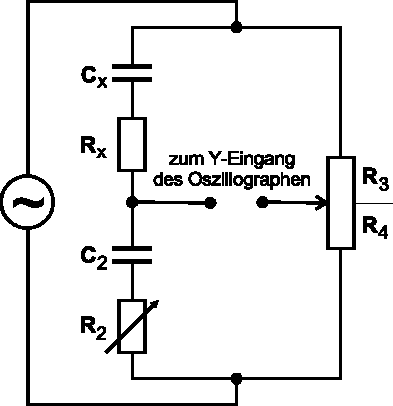
\includegraphics{figures/Kapazitätsmessbrücke.pdf}
    \caption{Kapazitätsmessbrücke\cite{ap07}.}
    \label{fig:kapamessbrü}
\end{figure}

$R_2$ stellt dabei ebenfalls einen variablen Widerstand dar, um die durch $R_x$ auftrende Phasenverschiebung zu kompensieren.
Es ergeben sich die Gleichungen
\begin{equation}
    R_x = R_2 \frac{R_3}{R_4}
    \label{eq:resxkapbrü}
\end{equation}
und 
\begin{equation}
    C_x = C_2 \frac{R_4}{R_3}
    \label{eq:kapxkapbrü}
\end{equation}
für den unbekannten Widerstand und die unbekannte Kapazität des Kondensators.


\subsection{Induktivitätsmessbrücke}
\label{subsec:indumessbrü}

Ähnlich zur Kapazitätsmessbrücke funktioniert auch die Messbrücke mit dem einzigen Unterschied, dass der Kondensator durch eine Spule der unbekannten Induktivität $I_x$ ersetzt wurde.
Auch hier müssen Wärmeverluste durch einen Widerstand $R_x$ kompensiert werden, die Schaltung gestaltet sich dann \autoref{fig:indumessbrü} entsprechend.

\begin{figure}[H]
    \centering
    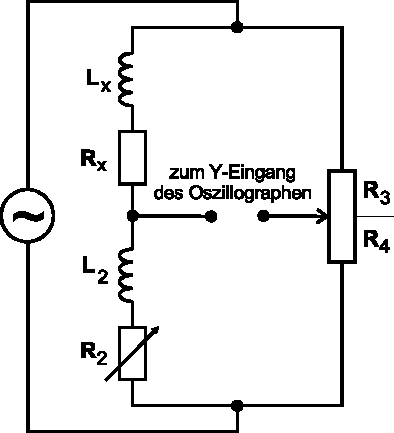
\includegraphics{figures/Induktivitätsmessbrücke.pdf}
    \caption{Induktivitätsmessbrücke für verlustbehaftete Spulen\cite{ap07}.}
    \label{fig:indumessbrü}
\end{figure}

Analog folgen hier

\begin{equation}
    R_x = R_2 \frac{R_3}{R_4}
    \label{eq:resxindubrü}
\end{equation}
und
\begin{equation}
    L_x = L_2 \frac{R_4}{R_3}\,.
    \label{eq:induxindubrü}
\end{equation}


\subsection{Maxwell-Brücke}
\label{subsec:maxwellbrü}

Alternativ lässt sich zur Bestimmung von Induktivitäten die in \autoref{fig:maxwellbrü} dargestellte
Schaltung verwendet.
Bei dieser wird als Ersatz zur Induktivität $L_2$ in der Induktivitätsmessbrücke ein Kondensator
der Kapazität $C_4$ gewählt, der Abgleich findet über $R_3$ und $R_4$ statt.

\begin{figure}[H]
    \centering
    \includegraphics{figures/Maxwell-Brücke.pdf}
    \caption{Maxwell-Brücke für verlustbehaftete Spulen\cite{ap07}.}
    \label{fig:maxwellbrü}
\end{figure}

Auch hier ergeben sich mit den bereits verwendeten Überlegungen

\begin{equation}
    R_x = R_2 \frac{R_3}{R_4}
    \label{eq:resxmaxwell}
\end{equation} für den unbekannten Verlustwiderstand und

\begin{equation}
    L_x = C_4 R_2 R_3
    \label{eq:induxmaxwell}
\end{equation} für die Induktivität der Spule.


\subsection{Wien-Robinson-Brücke}
\label{subsec:wienrobinson}

Die in \autoref{fig:wienrobinson} dargestellte Wien-Robinson-Brücke enthält keine Abgleichelemente, 
sondern dient als elektrischer Filter.
Sie entfernt die durch $ω_0 = \frac{1}{R C}$ gegebene Kreisfrequenz und schwächt die umliegenden 
Frequenzen stark ab. 

\begin{figure}[H]
    \centering
    \includegraphics{figures/Wien-Robinson-Brücke.pdf}
    \caption{Die Wien-Robinson-Brücke im Schaltbild\cite{ap07}.}
    \label{fig:wienrobinson}
\end{figure}

Mit $Ω = \frac{ω}{ω_0}$ gilt

\begin{equation}
    \left|\frac{U_{Br}}{U_S}\right|^2 = \frac{1}{9} \frac{(Ω^2 - 1)^2}{(1 - Ω^2) +9Ω^2} \,.
    \label{eq:omegadingens}
\end{equation}

Wird ein Sinusgenerator auf die auch Sperrfrequenz genannte Frequenz $ω_0$ eingestellt, bleiben nur
noch von $ω_0$ verschiedene Frequenzen übrig, die Summe ihrer Amplituden über die Restspannung messen.
Dieser \textbf{Oberwellengehalt} lässt sich durch den Klirrfaktor $k$ mit 
\begin{equation}
    k := \frac{\sqrt{U_2^2 + U_3^2 + ...}}{U_1}
    \label{eq:klirrfaktor}
\end{equation} darstellen, wobei $U_1$ die Amplitude der Grundwelle und $U_n$ die Amplitude der n-ten
Oberwelle der Frequenz $n ν_0$ ist.
Außerdem gilt
\begin{equation}
    U_2 = \frac{U_{Br}}{f(2)}\,,
    \label{eq:U2klirr}
\end{equation} dabei ist $f(2)$ die zu $U_2$ gehörige Frequenz.


%% Eigentlich fertig
